\title{SMARTFIN}
% Slide 1
\begin{frame}{SmartFin}
        \centering 
    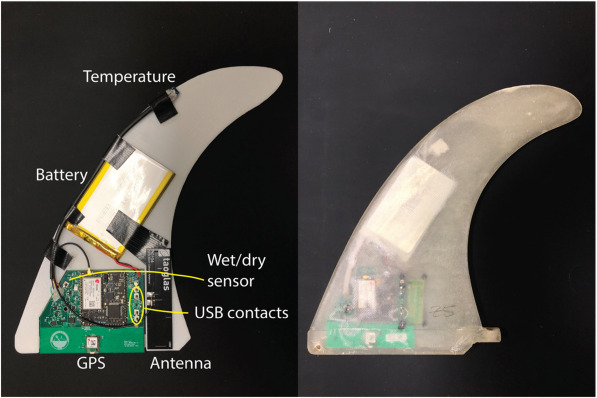
\includegraphics[width=0.8\textwidth, height=0.6\textheight, keepaspectratio]{images/labelled-smartfin.jpg}
    \vspace{0.5em} 
    \begin{itemize}
        \item Validate system with sensors.
        \item Primary Focus: IMU characterization.
    \end{itemize}
\end{frame}

% Slide 2
\begin{frame}{Key IMU Parameters}
    \centering
    \begin{tabular}{|l|l|}
        \hline
        \textbf{Parameter(s)} & \textbf{Sensor(s)} \\
        \hline
        Noise Density, Random Walk & A, G, M \\
        \hline
        IMU Orientation & A, G, M  \\
        \hline
        Scale Factor & Gyroscope \\
        \hline
    \end{tabular}
\end{frame}


% Slide 3
\begin{frame}{Expected Charts}
    \centering 
    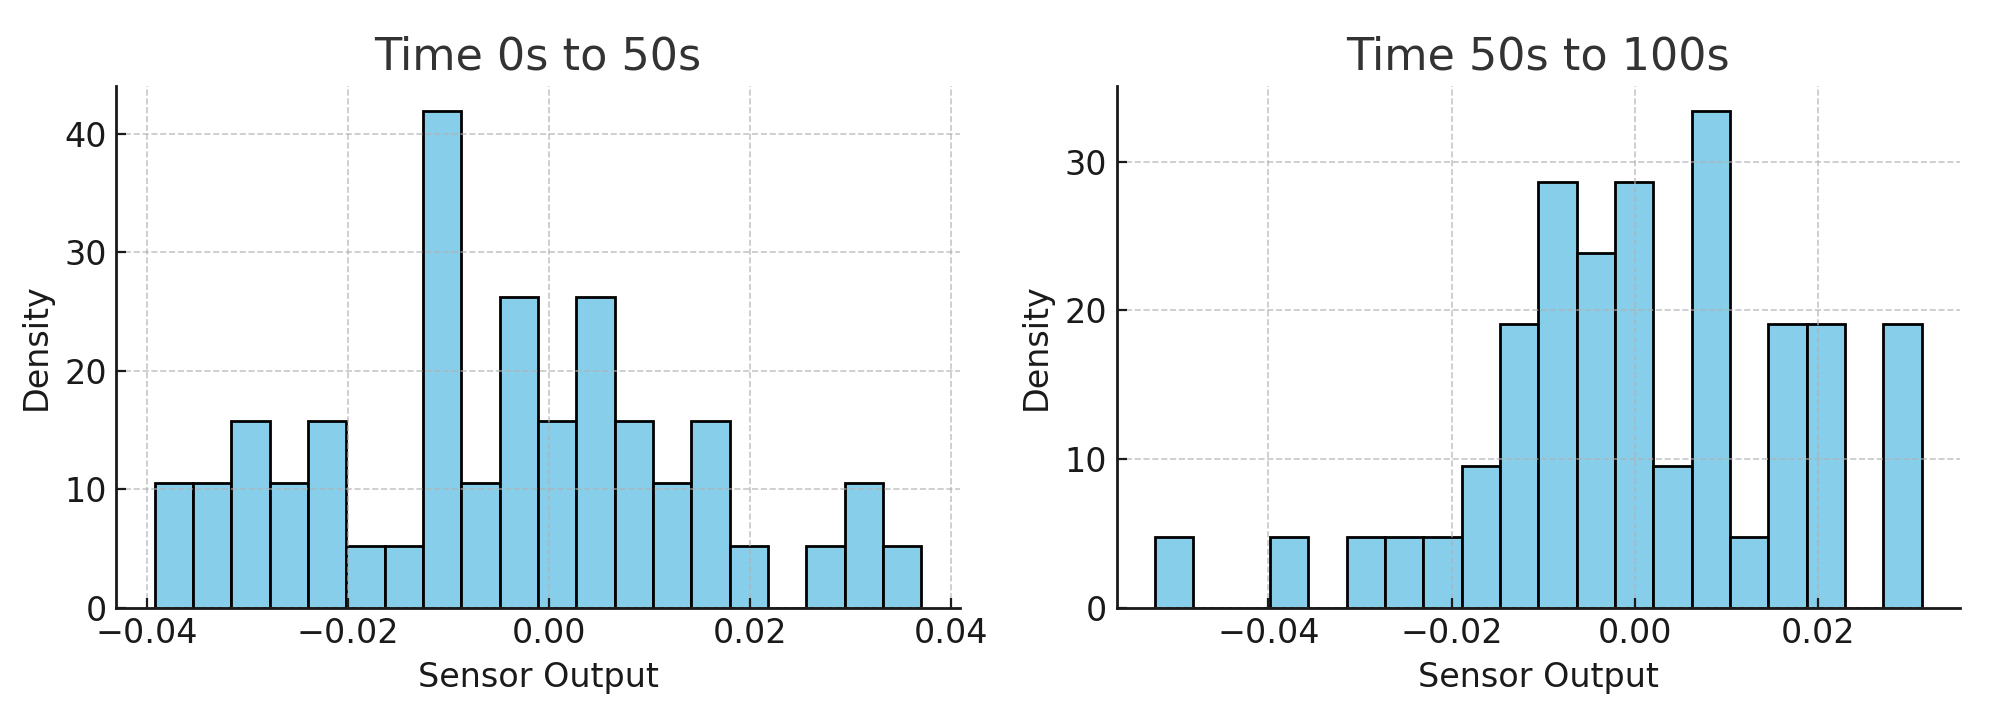
\includegraphics[width=1.0\textwidth, height=0.8\textheight, keepaspectratio]{images/imu-noise.png}
    \vspace{0.5em} 
    Distribution of sensor noise over time 
\end{frame}

% Slide 4
\begin{frame}{Expected Charts}
    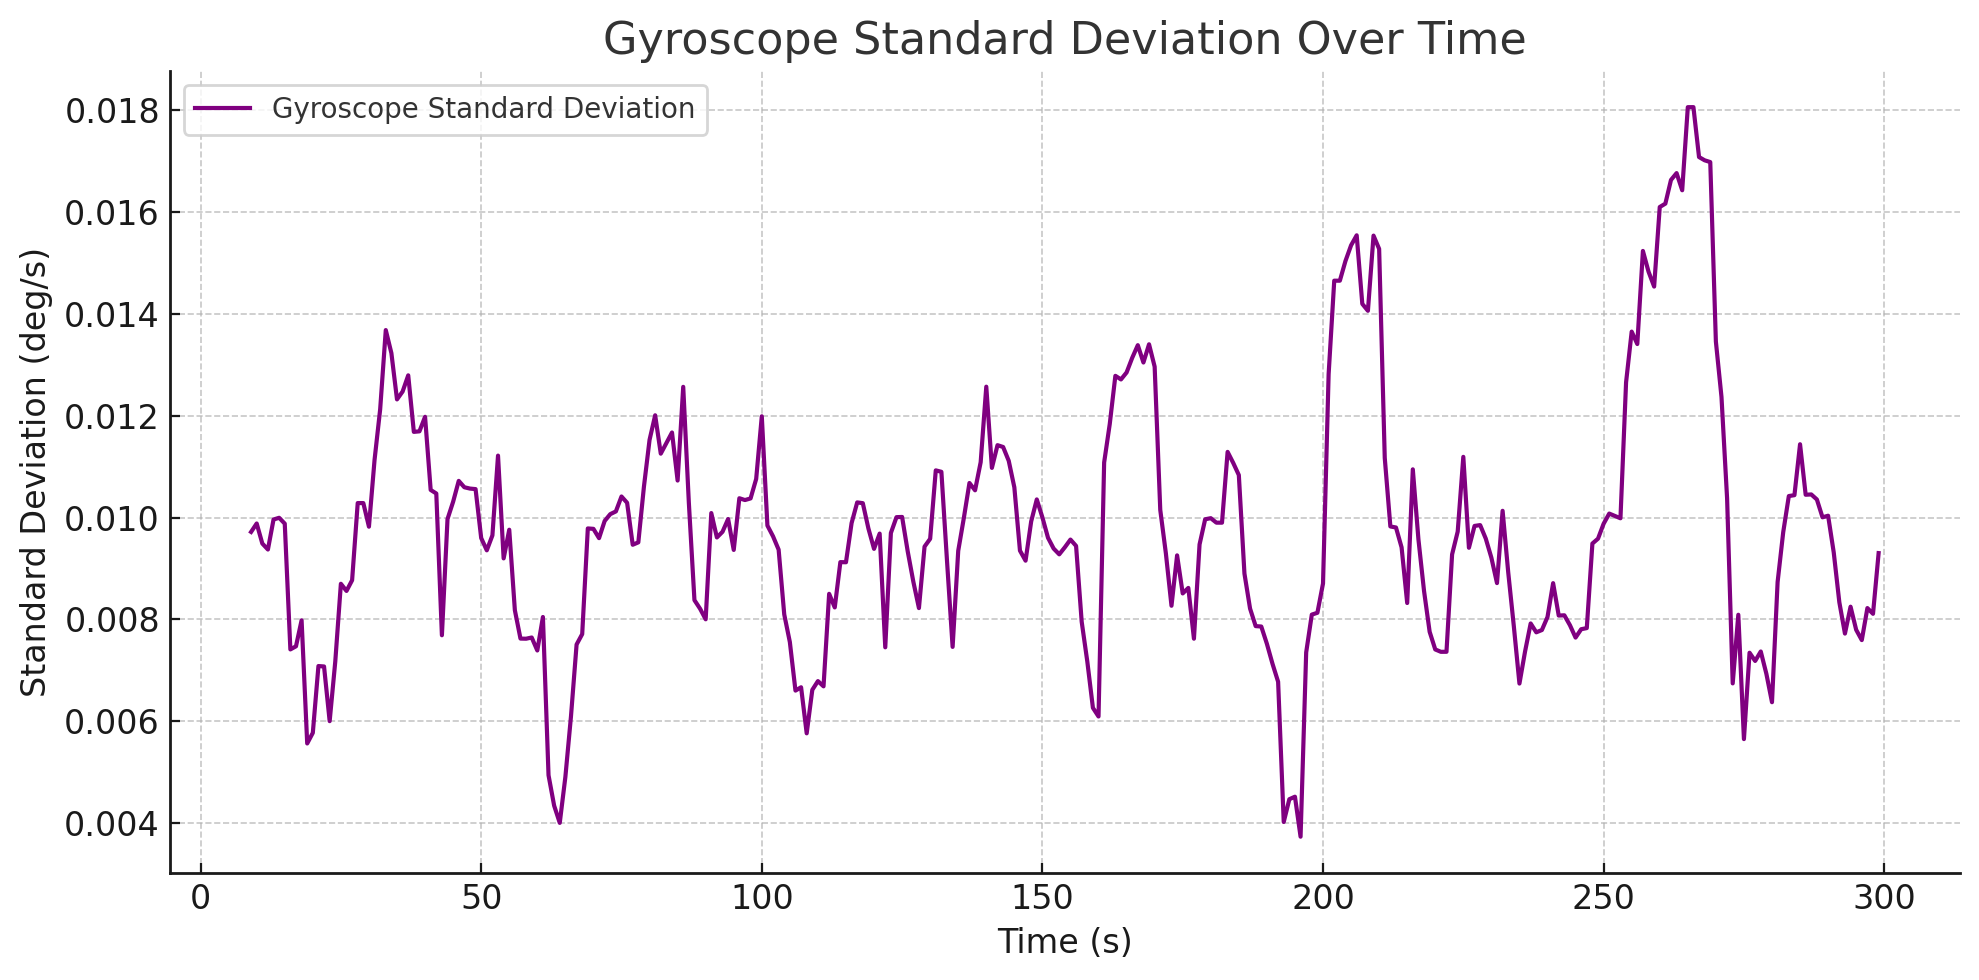
\includegraphics[width=1.0\textwidth, height=0.8\textheight, keepaspectratio]{images/gyroscope-chart.png}
    \vspace{0.5em} 
    Scale Factor - Gyroscope Temperature Change
\end{frame}

% Slide 5
\begin{frame}{Expected Charts}
     \centering 
    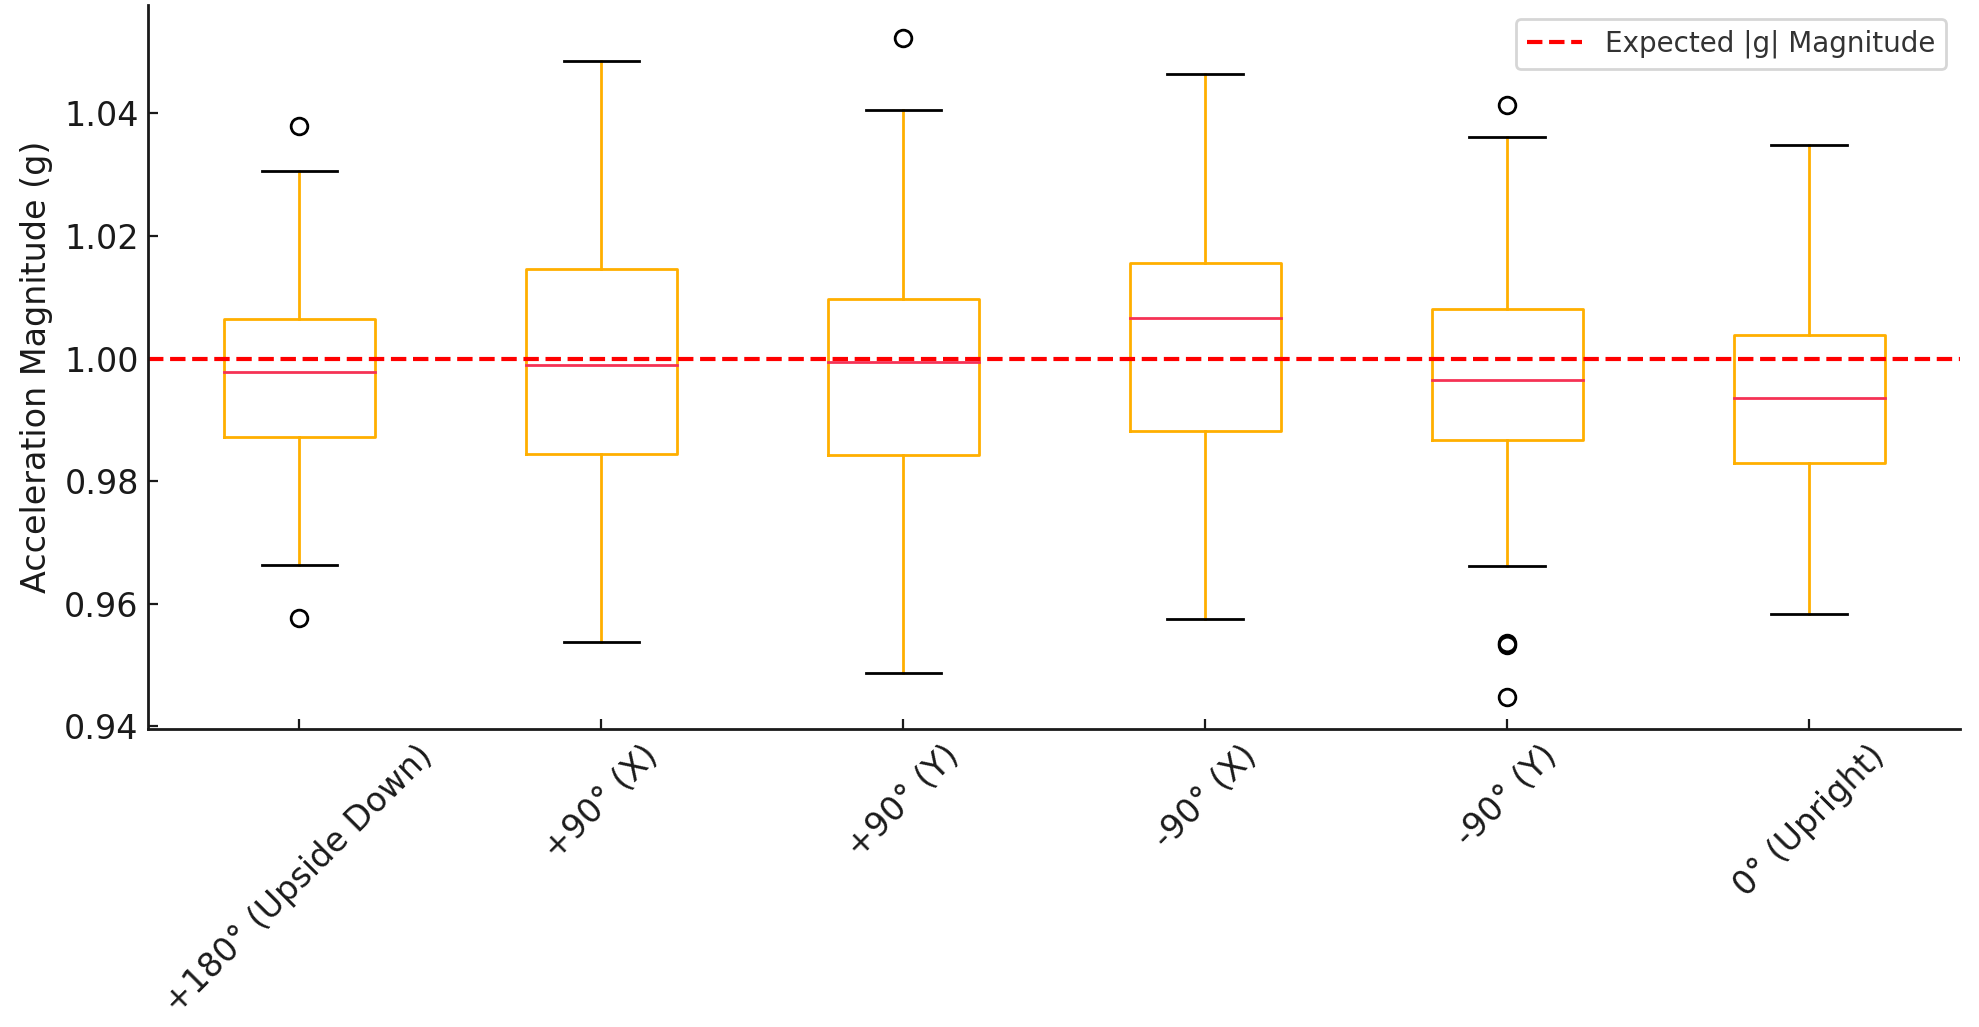
\includegraphics[width=1.0\textwidth, height=0.8\textheight, keepaspectratio]{images/orientation-boxplot.png}
    \vspace{0.5em} 
 Orientation: Box Plot (Measured vs Expected)
\end{frame}

% Slide 6
\begin{frame}{Implementation}
    \begin{itemize}
        \item Testing on Static Environment
        \item IMU Orientation 
    \end{itemize}
\end{frame}
